\documentclass[12pt, a4paper, twoside,openany,titlepage]{article}

% Inclusion of packages:

% The geometry package is used to alter the margins of each page
\usepackage[inner=5cm,outer=2cm,ignoreheadfoot,top=4cm,bottom=5cm,footskip=4cm]{geometry}
% the url package is used ot include URLs without messing up the rest
% of the latex
\usepackage[hyphens]{url}
% the graphicx package lets me include figures
\usepackage{graphicx}
% the listings package lets me include program listings
\usepackage{listings}
% the caption package lets me specify float caption properties
\usepackage[]{caption}
% the color package lets me define colors as strings
\usepackage{color}
% the url package lets me include urls
\usepackage{url}
% use package upquote to make all verbatim quotes straight quotes
\usepackage{upquote}
% the needspace package helps to keep command line block together
\usepackage{needspace}
%
\usepackage[hang,flushmargin,multiple,perpage]{footmisc}
%
\usepackage{fancyhdr}
% use package makeidx to create an index
\usepackage{makeidx}
% use package nameref to be able to refer to sections by name
\usepackage{nameref}

\makeindex

% Additional configuration:
\setlength{\captionmargin}{2.5cm}
\setlength{\parindent}{0pt}
\setlength{\parskip}{0.75em}
\setlength{\skip\footins}{2cm}

% define a bunch of color strings
\definecolor{gray}{rgb}{0.5,0.5,0.5}
\definecolor{lgray}{rgb}{0.9,0.9,0.9}
\definecolor{darkgray}{rgb}{0.15,0.15,0.15}
\definecolor{black}{rgb}{0,0,0}
\definecolor{white}{rgb}{1,1,1}

\lstdefinestyle{basic}{basicstyle=\scriptsize\ttfamily,
   numbersep=3mm,
   tabsize=4,
   showspaces=false,
   showstringspaces=false,
   frame=none,
   framexleftmargin=0mm,
   framexrightmargin=0mm,
   aboveskip = 0.5em,
   belowskip = -0.5em,
   xleftmargin = 0mm,
   breaklines = false,
}
\lstdefinestyle{bash}{basicstyle=\color{black}\scriptsize\ttfamily,
                      language=bash,
                      keywords={},
                      keywordstyle=\color{black},
                      commentstyle=\color{black},
                      stringstyle=\color{black},
                      backgroundcolor=\color{lgray}
}
\lstdefinestyle{Java}{basicstyle=\color{black}\scriptsize\ttfamily,
                      language=Java,
                      backgroundcolor=\color{lgray}
}


\newcommand{\mytilde}{\raise.17ex\hbox{$\scriptstyle\sim$}}


\fancypagestyle{plain}{%
\fancyhf{} % clear all header and footer fields
\renewcommand{\headrulewidth}{0pt}
\renewcommand{\headrulewidth}{0pt}
\fancyfoot[OC,EC]{--\ \thepage{}\ --}
}%fancypagestyle


\renewcommand{\captionfont}{\footnotesize}
\renewcommand{\captionlabelfont}{\sffamily}


\newcommand{\insertemptypage}[0]{
\vfill
\newpage
\thispagestyle{empty}
\mbox{}
\pagebreak
}



\author{Jurriaan H. Spaaks \and Jason Maassen}

\title{\textbf{Distributed Computing with Xenon} \\ tutorial}


\hyphenation{compiled}

\begin{document}

\maketitle

\insertemptypage{}

\pagestyle{plain}
\frontmatter

\tableofcontents
\insertemptypage{}

\mainmatter


\section{Introduction}

Many scientific applications require far more computation or data storage than can be handled on a regular PC or laptop. For such applications, access to remote storage and compute facilities is essential. Unfortunately, there is not a single standardized way to access these facilities. There are many competing protocols and tools in use by the various scientific data centers and commercial online providers.

As a result, application developers are forced to either select a few protocols they wish to support, thereby limiting which remote resources their application can use, or implement support for all of them, leading to excessive development time.

Xenon is a library designed to solve this problem. It offers a simple, unified programming interface to many remote computation and data storage facilities, and hides the complicated protocol and tool specific details from the application. By using Xenon, the application developer can focus on the application itself, without having to worry about which protocols to support, resulting in faster application development.

% TODO examples of what you can do with it

\subsection{Purpose of this document}

This document aims to help users without much prior knowledge about Java programming and without much experience in using remote systems to understand how to use the Xenon library.

\subsection{Version information}

It is assumed that you are using one of the Ubuntu-based operating systems (I'm using Linux Lubuntu 14.10). Nonetheless, most of the material covered in this manual should be usable on other Linux distributions with minor changes. The manual is written to be consistent with Xenon\url{@6d51d61}\footnote{commit \url{https://github.com/NLeSC/Xenon/tree/6d51d61}}.

\section{Conceptual overview}

% TODO explain the notion of files (files interface)
% TODO explain the notion of jobs (jobs interface)
% TODO explain the notion of credentials (credential interface)
% TODO explain the notion of adaptors

\begin{figure}[ht]
\centering
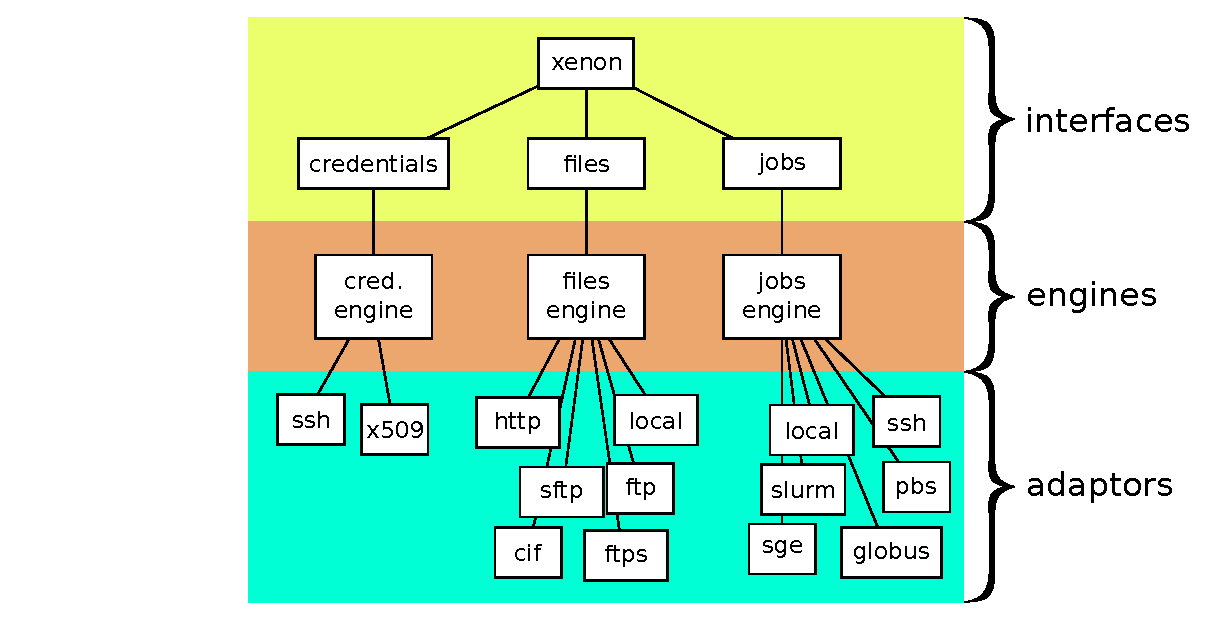
\includegraphics[width=1.0\columnwidth]{images/xenon-design}
\caption{\label{fig:xenon-design} Xenon is built on 3 pillars: `credentials'\index{Xenon!pillars!credentials}, `files'\index{Xenon!pillars!files} and `jobs'\index{Xenon!pillars!jobs}. Each pillar consists of an interface\index{Xenon!interface}, an engine\index{Xenon!engine}, and an adaptor\index{Xenon!adaptor}.}
\end{figure}


\section{Required software}
\index{Xenon!required software}

\needspace{6\baselineskip}
To use a minimal feature set of the Xenon library, you'll need the following software packages:
\begin{enumerate}
\item{\textit{Git}\index{Git}, a version management system;}
\item{\textit{Java}\index{Java}, a general purpose programming language;}
\item{\textit{Gradle}\index{Gradle}, a build automation system.}
\end{enumerate}


\needspace{10\baselineskip}
Additionally, you'll need to install (a subset of) the following packages if you want to use Xenon's full feature set, or when you want to help develop the library:
\begin{enumerate}
\item{\textit{Eclipse}\index{Eclipse}, an integrated development environment for Java, including the \textit{FindBugs}\index{Eclipse!FindBugs plugin} plugin for static code analysis;}
\item{\textit{Docker}\index{Docker}, a technology to execute programs in a container;}
\item{\textit{Texlive}\index{Texlive}, a \TeX{} type setting system. For Debian based OSs: texlive-latex-extra texlive-font-utils;}
\end{enumerate}

The following sections describe the necessary steps in more detail.

\subsection{Git}
\index{Git}

Open a terminal (default keybinding Ctrl + Alt + t). The shell should be Bash\index{Bash}. You can check this with:
\begin{lstlisting}[style=basic,style=bash]
echo $0
\end{lstlisting} % fix syntax highlighting by inserting an extra dollar sign $
which should return \texttt{/bin/bash}.

Now install \texttt{git}\index{Git!git@\texttt{git}} if you don't have it already:
\begin{lstlisting}[style=basic,style=bash]
sudo apt-get install git
\end{lstlisting}

After the install completes, we need to get a copy of the Xenon software. We will use \texttt{git} to do so. Change into the directory that you want to end up containing the top-level repository directory. I want to put the Xenon stuff in my home directory, so for me that means:
\begin{lstlisting}[style=basic,style=bash]
cd ${HOME}
\end{lstlisting} % fix syntax highlighting by inserting an extra dollar sign $
Then clone the Xenon repository into the current directory:
\begin{lstlisting}[style=basic,style=bash]
git clone https://github.com/NLeSC/Xenon.git
\end{lstlisting}
This will create a directory \texttt{\mytilde{}/Xenon} that contains the Xenon source code.

\subsection{Java}
\index{Java}

Xenon is a Java library, therefore it needs Java in order to run. Java comes in different versions identified by a name and a number. The labeling is somewhat confusing\footnote{See for example \url{http://stackoverflow.com/questions/2411288/java-versioning-and-terminology-1-6-vs-6-0-openjdk-vs-sun}}. This is partly because Java was first developed by Sun Microsystems (which was later bought by Oracle Corporation), while an open-source implementation is also available (it comes standard with many Linuxes). Furthermore, there are different flavors for each version, each flavor having different capabilities. For example, if you just want to \textit{run} Java applications, you need the JRE\index{JRE} (Java Runtime Environment\index{Java Runtime Environment}); if you also want to \textit{develop} Java software, you'll need either an SDK\index{SDK} (Software Development Kit\index{Java Software Development Kit}) from Sun/Oracle, or a JDK\index{JDK} (Java Development Kit\index{Java Development Kit}) if you are using the open-source variant.

Check if you have Java and if so, what version you have:
\begin{lstlisting}[style=basic,style=bash]
java -version
\end{lstlisting}
That should produce something like:
\begin{lstlisting}[style=basic,style=bash]
java version "1.7.0_79"
OpenJDK Runtime Environment (IcedTea 2.5.6) (7u79-2.5.6-0ubuntu1.14.04.1)
OpenJDK 64-Bit Server VM (build 24.79-b02, mixed mode)
\end{lstlisting}
Note that `Java version 1.7' is often referred to as `Java 7'.

If you don't have Java yet, install it with:
\begin{lstlisting}[style=basic,style=bash]
sudo apt-get install default-jdk
\end{lstlisting}


\subsection{Gradle}
\index{Gradle}

In order to use the source code from the library, we need to compile it first. Compiling source code can be a repetitive task, but fortunately there are tools available that automate much of the build process. Xenon uses Gradle for building the library.

Install Gradle using
\begin{lstlisting}[style=basic,style=bash]
sudo apt-get install gradle
\end{lstlisting}




\subsubsection{How Gradle uses conventions: an example}

In this section, I'll try to demonstrate how little configuration Gradle needs in order to be able to build Java projects successfully---as long as you don't deviate from existing conventions with regard to how the code is organized.

Make a new directory, for example \texttt{\mytilde{}/tmp/hellogradle}:
\begin{lstlisting}[style=basic,style=bash]
cd ${HOME}
mkdir -p tmp/hellogradle
\end{lstlisting} %$ dummy dollar


Then \texttt{cd} into the new directory and make a new subdirectory \texttt{src/main/java} in it. \texttt{src/main/java} is the conventional place where Java source code is stored.

\needspace{5\baselineskip}
Now open a text editor and copy-paste this Java class into it:
\begin{lstlisting}[style=basic,style=Java]
package nl.esciencecenter.hellogradle;

public class HelloGradle {

    public static void main(String[] args) {
        System.out.println("Hello, Gradle");
    }

}
\end{lstlisting}
And then save the Java class as \texttt{HelloGradle.java} in the newly created \texttt{src/main/java} directory. Files containing Java source code should have filenames that end in \url{.java}\index{Java!file extension!source code}\index{Java!file extension!.java@\texttt{.java}}.

Now let's make the simplest Gradle build file\index{Gradle!build file}. Open a new text editor and copy-paste this into it:
\begin{lstlisting}[style=basic,style=bash]
apply plugin: 'java'
\end{lstlisting}
Then save as \texttt{build.gradle}\index{Gradle!build.gradle@\texttt{build.gradle}} (the default name for Gradle build files) in the \texttt{\mytilde{}/tmp/hellogradle} directory. At this point, \texttt{\mytilde{}/tmp/hellogradle} should contain this:
\begin{lstlisting}[style=basic,style=bash]
build.gradle
src
src/main
src/main/java
src/main/java/HelloGradle.java
\end{lstlisting}

The \texttt{apply plugin}\index{Gradle!apply plugin@\texttt{apply plugin}} line in \texttt{build.gradle} tells Gradle to use the Java plugin for Gradle\index{Gradle!Java plugin}. The Java plugin defines a number of build tasks typical for a Java project. It also specifies the default locations for the project's Java source code (\texttt{src/main/java}), the compiled Java classes (\texttt{build/classes}), the documentation (\texttt{build/docs/javadoc}), as well as some other things that we'll check out later, such as unit testing and integration testing. You can find the details online at \url{https://docs.gradle.org/current/userguide/java_plugin.html}.

Gradle can tell you what tasks it knows about. Try running
\begin{lstlisting}[style=basic,style=bash]
cd ${HOME}/tmp/hellogradle
gradle --build-file build.gradle tasks
\end{lstlisting} %$ (dummy dollar)
The \texttt{--build-file} option is used to specify which file to use as input to gradle; its short version is \texttt{-b}. This will give you the default tasks that Gradle knows about, such as \texttt{help} and \texttt{properties}. Note that \texttt{tasks} itself is a task, and so it is listed along with the other tasks. Additionally, it will list any tasks that are defined in \texttt{build.gradle}. Note that this includes any tasks which are defined implicitly (for example by \texttt{apply plugin} lines). To get a little more information on each task's dependencies, you can add the \texttt{--all} option as follows:
\begin{lstlisting}[style=basic,style=bash]
cd ${HOME}/tmp/hellogradle
gradle --build-file build.gradle tasks --all
\end{lstlisting} %$ (dummy dollar)

In the output, there should be a task called \texttt{classes}, which compiles the (main) source code. The task \texttt{classes} is added by the Java plugin. Let's build our \url{src/main/java/HelloGradle.java} and see what that gives us. Run:
\begin{lstlisting}[style=basic,style=bash]
cd ${HOME}/tmp/hellogradle
gradle --build-file build.gradle classes
\end{lstlisting} %$ dummy dollar
Afterwards, the directory should contain the following files and directories:
\begin{lstlisting}[style=basic,style=bash]
build
build/classes
build/classes/main
build/classes/main/nl
build/classes/main/nl/esciencecenter
build/classes/main/nl/esciencecenter/hellogradle
build/classes/main/nl/esciencecenter/hellogradle/HelloGradle.class
build/dependency-cache
build.gradle
src
src/main
src/main/java
src/main/java/HelloGradle.java
\end{lstlisting}
As you can see, Gradle generated a directory \texttt{build} and put all the things it built in it. It created a subdirectory \texttt{classes}, containing yet another subdirectory \texttt{main}, since that is the name of the so-called \mbox{`sourceSet'}\index{sourceSet} (a collection of source code files that belong together conceptually). Inside \texttt{main}, there are nested subdirectories for each part of the package name \url{nl.esciencecenter.hellogradle}. Finally, there is the compiled Java class \texttt{HelloGradle.class}. Note that files containing compiled Java code should have filenames that end in \url{.class}\index{Java!file extension!compiled}\index{Java!file extension!.class@\texttt{.class}}.
% TODO add a line about dependency-cache

Let's see if the compile worked. Run
\begin{lstlisting}[style=basic,style=bash]
cd ${HOME}/tmp/hellogradle
java -classpath build/classes/main nl.esciencecenter.hellogradle.HelloGradle
\end{lstlisting} %$ (dummy dollar to fix editor highlighting)
The \texttt{-classpath} option tells Java it should look in \url{build/classes/main} for compiled Java classes (its short option name is \texttt{-cp}). The last argument, \url{nl.esciencecenter.hellogradle.HelloGradle} is the fully qualified name of the class we want to run. If everything worked, you should see the `Hello Gradle' greeting.

\vspace{2em}
\textit{Javadoc}
\index{Javadoc}\index{Java!Javadoc}

Java comes with a neat system of automatically documenting source code, called `Javadoc'. Javadoc is able to parse the Java source code, analyzing its structure for things like class hierarchy, public interfaces, public class methods, constructors, etc. Javadoc then generates the corresponding documentation automatically. The great advantage of generating the documentation in an automated way \textit{from the source code} is that the documentation is always up to date with how the code works.

Thanks to the Java plugin, Gradle knows how to generate Javadoc (if you run \texttt{gradle --build-file build.gradle tasks} again, you'll see a task \texttt{javadoc}, which as the name suggests, generates Javadoc documentation. You can run the \texttt{javadoc} task in the same way as you run any other task:
\begin{lstlisting}[style=basic,style=bash]
cd ${HOME}/tmp/hellogradle
gradle --build-file build.gradle javadoc
\end{lstlisting} %$ (dummy dollar to fix editor highlighting)

The \texttt{build} directory should now have a few new items:
\begin{lstlisting}[style=basic,style=bash]
build
build/docs
build/docs/javadoc
build/docs/javadoc/nl
build/docs/javadoc/nl/esciencecenter
build/docs/javadoc/nl/esciencecenter/hellogradle
build/docs/javadoc/nl/esciencecenter/hellogradle/package-summary.html
build/docs/javadoc/nl/esciencecenter/hellogradle/HelloGradle.html
build/docs/javadoc/nl/esciencecenter/hellogradle/package-frame.html
build/docs/javadoc/nl/esciencecenter/hellogradle/package-tree.html
build/docs/javadoc/deprecated-list.html
build/docs/javadoc/constant-values.html
build/docs/javadoc/allclasses-noframe.html
build/docs/javadoc/overview-tree.html
build/docs/javadoc/index.html
build/docs/javadoc/help-doc.html
build/docs/javadoc/index-all.html
build/docs/javadoc/stylesheet.css
build/docs/javadoc/resources
build/docs/javadoc/resources/background.gif
build/docs/javadoc/resources/tab.gif
build/docs/javadoc/resources/titlebar_end.gif
build/docs/javadoc/resources/titlebar.gif
build/docs/javadoc/allclasses-frame.html
build/docs/javadoc/package-list
build/tmp
build/tmp/javadoc
build/tmp/javadoc/javadoc.options
build/classes
build/classes/main
build/classes/main/nl
build/classes/main/nl/esciencecenter
build/classes/main/nl/esciencecenter/hellogradle
build/classes/main/nl/esciencecenter/hellogradle/HelloGradle.class
build/dependency-cache
build.gradle
src
src/main
src/main/java
src/main/java/HelloGradle.java
\end{lstlisting}

You can use any web browser to navigate through the Javadoc documentation (\url{build/docs/javadoc/index.html} is probably the best starting point).

Gradle also defines a task to clean up the directory, such that you only have the bare essentials. This task is called \texttt{clean} and can be run with
\begin{lstlisting}[style=basic,style=bash]
gradle --build-file build.gradle clean
\end{lstlisting}


Note that in order to generate the documentation, the source needed to be compiled first. The task \texttt{javadoc} is said to \textit{depend on} the task \texttt{classes}. You can check that this is indeed the case by:
\begin{lstlisting}[style=basic,style=bash]
gradle --build-file build.gradle javadoc
\end{lstlisting}
This should generate \url{build/docs/javadoc} as before, but only after generating \url{build/classes} first.


So far, we've been explicitly specifying what build file Gradle should use through \texttt{gradle}'s \url{--build-file} option. However, as long as you are using the default build file (\texttt{build.gradle}), there's no need to be explicit about that---you can just run \texttt{gradle} followed by the name of the task, e.g.:
\begin{lstlisting}[style=basic,style=bash]
gradle javadoc
\end{lstlisting}

While Javadoc's automated documentation generation is helpful when it comes to the \textit{how} of the Java code, it can provide little in terms of the \textit{why} (or the \textit{why like this}). The solution for that particular problem necessarily requires input from the programmer. That is, the programmer can clarify his/her Java code by including Javadoc directives (\textit{tags}\index{Javadoc!tags}\index{Java!Javadoc!tags}), which can help explain the meaning of input arguments, variables, methods, classes, and so forth. The most common tags are listed in Table~\ref{tab:javadoc-tags}.


\begin{table}[!ht]
\vspace{1em}
\caption{Commonly used Javadoc tags.\label{tab:javadoc-tags}}
\begin{tabular}{lp{10cm}}
\vspace{0.5em}
\textbf{Tag name}    & \textbf{What the tag does}                                 \\
\texttt{@author}     & Specifies the author(s).                                   \\
\texttt{@version}    & Specifies the version.                                     \\
\texttt{@param}      & Describes a method parameter.                              \\
\texttt{@return}     & Describes the (meaning of the) returned value.             \\
\texttt{@throws}     & Describes what exceptions are thrown by this method.       \\
\texttt{@see}        & Provides a link to another element of the documentation.   \\
\texttt{@link}       & References a place in the javadoc.                         \\
\texttt{@deprecated} & Advises the user not to use a program element anymore, and ideally specifies what to use instead.     \\
\texttt{@since}      & Specifies when certain functionality was first introduced. \\
\end{tabular}
\end{table}

Note that by convention the tags appear in this order, and that Javadoc tags are lowercase.

Personally, I think \texttt{@author} is probably best avoided---if you want to know who contributed what, ask the version management system. For example, if you have a file \url{UnknownPropertyException.java} and you use \texttt{git} for version management, entering \texttt{git blame UnknownPropertyException.java}\index{Git!git blame@\texttt{git blame}} at the command line will give you a line-by-line overview of who commited what, when. Online code repositories such as Github typically also provide this capability in the form of a \textit{blame button}.
%Similarly, \texttt{@version} and \texttt{@since} are also best avoided, since the notion of versions is a little bit outdated or at least inconsistent with how Git works.
You may use \texttt{@author unascribed} if you do not want to, or cannot specify the author.

As a small example, update \url{HelloGradle.java} with a Javadoc comment, explaining what this class does, as follows:
\begin{lstlisting}[style=basic,style=bash]
package nl.esciencecenter.hellogradle;

/**
 *  This is a short one-line description of the class.
 *  <p>
 *  The Javadoc comment block appears just before the class
 *  it describes.
 *  </p>
 *  <p>
 *  You could use another paragraph to explain more stuff.
 *  </p>
 *
 *  @author      Firs T. Author
 *  @author      Secon D. Author
 *  @version     1.0, 9-Sept-2015
 *  @deprecated  As of release 1.3, replaced
 *               by {@link nl.esciencecenter.ByeGradle}
 */
public class HelloGradle {

    /**
    * 'main' is the only method.
    */
    public static void main(String[] args) {
        System.out.println("Hello, Gradle");
    }

}
\end{lstlisting}

Now run \texttt{gradle javadoc} again and check how that changed \url{build/docs/javadoc/index.html}.

\needspace{5\baselineskip}
Note that Javadoc expects the commenting style to be exactly like this:
\begin{lstlisting}[style=basic,style=bash]
/**  <- javadoc opening tag
 *  (any number of lines like this line)
 */  <- javadoc closing tags
\end{lstlisting}

% TODO add gradle eclipse


\subsubsection{The Gradle wrapper}
% TODO gradlew see https://spring.io/guides/gs/gradle/

% TODO what is the gradle wrapper

So far, we've been calling the \texttt{gradle} executable directly. There is, however, a better way of starting a Gradle build, namely by using the so-called `Gradle wrapper'\index{Gradle!wrapper}. The Gradle wrapper consists of a shell script (\url{gradlew}), a configuration file (\url{gradle/wrapper/gradle-wrapper.properties}), and some compiled Java code bundled into a Java archive (\url{gradle/wrapper/gradle-wrapper.jar}).

The Gradle wrapper is the preferred way of starting a Gradle build. This is because using \texttt{./gradlew}\index{Gradle!gradlew@\texttt{gradlew}} offers a couple of advantages over using \texttt{gradle}\index{Gradle!gradle@\texttt{gradle}}.
%
Firstly, users don't need to install Gradle in order to build the software. This is particularly convenient when  building the software on machines that are not owned or maintained by the user, as is typically the case during \textit{continuous integration testing}\index{continuous integration testing} using software such as Jenkins\index{Jenkins} or Travis\index{Travis}; we'll take a look at testing later.
%
Secondly, using the Gradle wrapper gives you the option of running a Gradle version which is more up-to-date than what's available in the operating system's software repositories. For example, my Lubuntu 14.10 comes with Gradle version 1.4, while Gradle is currently at version 2.7.
%
Thirdly, since the Gradle wrapper files are checked into the version control system, they become part of the software. This ensures that software users are running the exact same build setup as are the software developers, which improves the robustness of the software when everything is running smoothly, and improves reproducability when bugs occur.
% TODO explain first-time plugin download and where those plugins are stored
% TODO clean caches: rm ~/.m2 (maven stuff) and ~/.gradle/caches (gradle stuff)


\subsubsection{Building Xenon with Gradle}

\index{Xenon!Gradle!online building}
Normally, you'd build Xenon while connected to the Internet. Gradle then downloads whatever additional software it needs. Gradle will first try to download such packages from MavenCentral\footnote{\url{https://repo1.maven.org/maven2}} (\index{MavenCentral}a website that hosts many common Java packages, in many different versions); if the package is not available from MavenCentral, or if the download fails for some other reason, Gradle tries a different website (Bintray\index{Bintray}\index{JCenter}\footnote{\url{https://bintray.com/bintray/jcenter}}). The \texttt{repositories} section in \texttt{build-common.gradle} lists the repositories that Gradle will try to connect to.

\index{Xenon!Gradle!offline building}
It is also possible to build Xenon while disconnected from the Internet, but in order for that to work, you need to have run \texttt{./gradlew} at least once before (while connected to the Internet). This ensures that the necessary Gradle plugins, as well as any libraries that Xenon is dependant on, will have been downloaded.
% NEEDS_VERIFICATION the local copy only exists if this is not the first time you build?
% NEEDS_VERIFICATION MavenCentral only for Java packages

In order to facilitate both online and offline building, we chose to divide the Gradle work over three files, located in the root of the repository:
\begin{enumerate}
\item{\texttt{build.gradle}\index{Xenon!Gradle!build.gradle@\texttt{build.gradle}} }
\item{\texttt{build-offline.gradle}} \index{Xenon!Gradle!build-offline.gradle@\texttt{build-offline.gradle}}}
\item{\texttt{build-common.gradle}} \index{Xenon!Gradle!build-common.gradle@\texttt{build-common.gradle}}}
\end{enumerate}

\texttt{build.gradle} and \texttt{build-offline.gradle} can be called directly as argument to \texttt{./gradlew} (or \texttt{gradle}, for that matter); \texttt{build-common.gradle} is not intended to be called directly (it should only get called from within either \texttt{build.gradle} or \texttt{build-offline.gradle}, through the use of \texttt{apply from}\index{Xenon!Gradle!apply from@\texttt{apply from}} lines. Deferring to \texttt{build-common.gradle} avoids duplication of any tasks that are the same, regardless of whether the build is offline or online.


\subsection{Verifying the software setup}


In this section, we will test the software setup by running a small example, \texttt{CreatingXenon}. \texttt{CreatingXenon} establishes a connection to a remote system, does something simple, and returns.
% FIXME add better description of what CreatingXenon does

\subsubsection{Checking the connectivity}

Before we can run the \texttt{CreatingXenon} example, we first have to make sure that we have access to a remote system. You'll need an account on the remote machine. For example, I have an account \texttt{jspaaks} on SURFsara's Lisa clustercomputer. Cluster computers typically have a dedicated machine (the so-called `headnode') that serves as the main entry point when connecting from outside the cluster. For Lisa, the headnode is located at \url{lisa.surfsara.nl}.

I can connect to Lisa's head node using the \texttt{ssh} command line program as follows:
\begin{lstlisting}[style=basic,style=bash,escapeinside={(*@}{@*)}]
# (my account on Lisa is called jspaaks)
ssh jspaaks@lisa.surfsara.nl
\end{lstlisting}

If this is the first time you connect to the remote machine, it will generally ask if you want to add the remote machine to the list of `known hosts'. For example, here's what the Lisa system tells me when I try to ssh to it:
\begin{lstlisting}[style=basic,style=bash,escapeinside={(*@}{@*)}]
The authenticity of host 'lisa.surfsara.nl (145.100.29.210)' can't be
established.
RSA key fingerprint is b0:69:85:a5:21:d6:43:40:bc:6c:da:e3:a2:cc:b5:8b.
Are you sure you want to continue connecting (yes/no)?
\end{lstlisting}
If I then type \texttt{yes}, it says\footnote{SURFsara publish RSA key fingerprints for their systems at \url{https://userinfo.surfsara.nl/systems/shared/ssh}. The number posted there should be the same as what you have in your terminal.}:
\begin{lstlisting}[style=basic,style=bash,escapeinside={(*@}{@*)}]
Warning: Permanently added 'lisa.surfsara.nl,145.100.29.210' (RSA) to
         the list of known hosts.

                             (*@\textit{<some content omitted>}@*)
\end{lstlisting}
and asks for my password.

The result of this connection is that you should now have a (hidden) directory \texttt{.ssh} in your \texttt{/home} directory, which should contain 3 files: \texttt{id\_rsa}, which contains your private RSA key(s); \texttt{id\_rsa.pub}, which contains your public RSA key(s); and \texttt{known\_hosts}, which contains a list of systems that you have successfully connected to in the past. \url{known_hosts} uses one line per known system, and each line begins with the following elements:
\begin{itemize}
\item{\texttt{1} a flag signifying that the third element (host name) is hashed using the SHA1 algorithm;}
\item{\texttt{x5PcOam9hhAjdF84++EKwodUNgQ} the (public) salt used to encrypt the host name;}
\item{\texttt{NK1rAZev7rV6JSTIdM3ymPpKlQ0}} the (hashed) host name;}
\item{key-value pairs, e.g. the RSA fingerprint of the Lisa system \url{ssh-rsa} \url{b0:69:85:a5:21:d6:43:40:bc:6c:da:e3:a2:cc:b5:8b}.}
\end{itemize}
Xenon uses \texttt{known\_hosts} to automatically connect to a (known) remote system, without having to ask for credentials every time.


\subsubsection{Simple Xenon program from the command line}

Now for the actual example. The sourceSet `main'\index{Xenon!sourceSet!main@\texttt{main}} contains the source code for Xenon. It is located at \url{src/main/java}. We'll also need a second sourceSet, `examples'\index{Xenon!sourceSet!examples@\texttt{examples}}, which contains the source code for the Xenon examples. We'll need to compile both sourceSets in order to run a simple Xenon Java program.

Let's first check what tasks we have by:
\begin{lstlisting}[style=basic,style=bash,escapeinside={(*@}{@*)}]
cd ${HOME}/Xenon
./gradlew tasks --all
\end{lstlisting} % dummy $

Under `Build tasks', there should be an item \texttt{examplesClasses}, used for compiling the `examples' sourceSet; \texttt{examplesClasses} has a dependent task \texttt{classes}, used for compiling the `main' sourceSet.

Running
\begin{lstlisting}[style=basic,style=bash,escapeinside={(*@}{@*)}]
cd ${HOME}/Xenon
./gradlew examplesClasses
\end{lstlisting} % dummy $
should give you a new directory \mytilde\url{/Xenon/build} with subdirectories \url{classes/examples} and {\url{classes/main} (as well as some other stuff).


The general syntax for running compiled Java programs from the command line\index{Java!from the command line} is as follows:
\begin{lstlisting}[style=basic,style=bash,escapeinside={(*@}{@*)}]
java (*@\textit{<fully qualified classname>}@*)
\end{lstlisting}
The fully qualified classname for our example is \url{nl.esciencecenter.xenon.examples.CreatingXenon}, but if you try to run
\begin{lstlisting}[style=basic,style=bash,escapeinside={(*@}{@*)}]
cd ${HOME}/Xenon
java nl.esciencecenter.xenon.examples.CreatingXenon
\end{lstlisting} % dummy $
you will get the error below:
\begin{lstlisting}[style=basic,style=bash,escapeinside={(*@}{@*)}]
Error: Could not find or load main class \
nl.esciencecenter.xenon.examples.CreatingXenon
\end{lstlisting}

This is because the \url{java} executable tries to locate our class \url{nl.esciencecenter.xenon.examples.CreatingXenon}, but we haven't told \url{java} where to look for it. We can resolve that by specifying a list of one or more directories using \texttt{java}'s classpath option \texttt{-cp}\index{Java!from the command line!classpath}\index{Java!from the command line!-cp@\texttt{-cp}}. There are 3 locations that are relevant for running \url{CreatingXenon}. These are:
\begin{enumerate}
\item{the location of \url{CreatingXenon} itself:\\ \mytilde\url{/Xenon/build/classes/examples}}
\item{the location of the Xenon classes:\\ \mytilde\url{/Xenon/build/classes/main}}
\item{the location of any libraries that Xenon depends on:\\ \mytilde\url{/Xenon/lib}}
\end{enumerate}
These directories can be passed to \texttt{java} as a colon-separated list. Directory names can be relative to the current directory. Furthermore, the syntax is slightly different depending on what type of file you want \texttt{java} to find in a given directory: if you want \texttt{java} to find compiled Java classes, use the directory name; if you want \texttt{java} to find jar files, use the directory name followed by \texttt{/*}. Finally, the order within the classpath is significant.
% TODO find out about the order in java classpath

Using paths relative to \mytilde\url{/Xenon} for items (1) and (2) above, and using the \texttt{/*} addition for item (3) yields the following classpath value for our example: \url{build/classes/examples:build/classes/main:lib/*}, so the whole command becomes:
\begin{lstlisting}[style=basic,style=bash,escapeinside={(*@}{@*)}]
cd ${HOME}/Xenon
java -cp build/classes/examples:build/classes/main:lib/* \
nl.esciencecenter.xenon.examples.CreatingXenon
\end{lstlisting} % dummy $



Your output should look something like this:
\begin{lstlisting}[style=basic,style=bash,escapeinside={(*@}{@*)}]
13:21:15.594 [Thread-0] DEBUG n.e.xenon.engine.util.CopyEngine - CopyEngin ...
13:21:15.606 [main] DEBUG n.e.xenon.engine.util.JobQueues - Creating JobQu ...
13:21:15.618 [main] DEBUG n.e.xenon.adaptors.ssh.SshAdaptor - Setting ssh  ...
13:21:15.632 [main] DEBUG n.e.xenon.adaptors.ssh.SshAdaptor - Host keys in ...
13:21:15.643 [main] DEBUG n.e.xenon.adaptors.ssh.SshAdaptor - |1|x5PcOam9h ...
13:21:15.650 [main] DEBUG n.e.xenon.adaptors.ssh.SshAdaptor -
13:21:15.650 [main] DEBUG n.e.xenon.adaptors.ssh.SshAdaptor - Setting ssh  ...
13:21:15.657 [main] WARN  n.e.xenon.adaptors.ssh.SshAdaptor - OpenSSH conf ...
java.io.FileNotFoundException: /home/daisycutter/.ssh/config (No such file or directory)
    at java.io.FileInputStream.open(Native Method) ~[na:1.7.0_79]
    at java.io.FileInputStream.<init>(FileInputStream.java:146) ~[na:1.7.0_79]
    at java.io.FileInputStream.<init>(FileInputStream.java:101) ~[na:1.7.0_79]
    at com.jcraft.jsch.Util.fromFile(Util.java:492) ~[jsch-0.1.50.jar:na]
    at com.jcraft.jsch.OpenSSHConfig.parseFile(OpenSSHConfig.java:97) ~[jsch-0.1.50.jar:na]
    at nl.esciencecenter.xenon.adaptors.ssh.SshAdaptor.setConfigFile(SshAdaptor.java:192) [main/:na]
    at nl.esciencecenter.xenon.adaptors.ssh.SshAdaptor.<init>(SshAdaptor.java:164) [main/:na]
    at nl.esciencecenter.xenon.adaptors.ssh.SshAdaptor.<init>(SshAdaptor.java:141) [main/:na]
    at nl.esciencecenter.xenon.engine.XenonEngine.loadAdaptors(XenonEngine.java:182) [main/:na]
    at nl.esciencecenter.xenon.engine.XenonEngine.<init>(XenonEngine.java:169) [main/:na]
    at nl.esciencecenter.xenon.engine.XenonEngine.newXenon(XenonEngine.java:92) [main/:na]
    at nl.esciencecenter.xenon.XenonFactory.newXenon(XenonFactory.java:57) [main/:na]
    at nl.esciencecenter.xenon.examples.CreatingXenon.main(CreatingXenon.java:39) [examples/:na]
Exception in thread "main" java.lang.NoClassDefFoundError: org/globus/tools/proxy/GridProxyModel
    at nl.esciencecenter.xenon.adaptors.gftp.GftpAdaptor.<clinit>(GftpAdaptor.java:47)
    at nl.esciencecenter.xenon.engine.XenonEngine.loadAdaptors(XenonEngine.java:187)
    at nl.esciencecenter.xenon.engine.XenonEngine.<init>(XenonEngine.java:169)
    at nl.esciencecenter.xenon.engine.XenonEngine.newXenon(XenonEngine.java:92)
    at nl.esciencecenter.xenon.XenonFactory.newXenon(XenonFactory.java:57)
    at nl.esciencecenter.xenon.examples.CreatingXenon.main(CreatingXenon.java:39)
Caused by: java.lang.ClassNotFoundException: org.globus.tools.proxy.GridProxyModel
    at java.net.URLClassLoader$1.run(URLClassLoader.java:366)
    at java.net.URLClassLoader$1.run(URLClassLoader.java:355)
    at java.security.AccessController.doPrivileged(Native Method)
    at java.net.URLClassLoader.findClass(URLClassLoader.java:354)
    at java.lang.ClassLoader.loadClass(ClassLoader.java:425)
    at sun.misc.Launcher$AppClassLoader.loadClass(Launcher.java:308)
    at java.lang.ClassLoader.loadClass(ClassLoader.java:358)
    ... 6 more
\end{lstlisting} % dummy $ %to fix syntax highlighting
% FIXME OpenSSH config file cannot be read error

\section{Optional software}
\index{Xenon!optional software}

This section describes the software you'll need if you not only want to run Xenon software, but also develop it.


\subsection{Eclipse}

Eclipse\index{Eclipse} is a very powerful, free, open-source, integrated development environment for Java (and many other languages). It is available in most Linuxes from their respective repositories. By default, Eclipse comes with many features, such as Git (version control)\index{Git}, Mylyn (task management)\index{Mylyn}, Maven (building)\index{Maven}, Ant (building)\index{Ant}, an XML editor, as well as some other stuff. While these features are nice, they can get in the way if you're new to code development with Java using Eclipse. We will therefore set up a minimal Eclipse installation which includes only the Eclipse platform and the Java related tools (most importantly, the debugger). Feel free to skip this next part if you're already familiar with Eclipse.

\subsubsection{A minimal Eclipse installation}
\index{Eclipse!minimal installation}

Go to \url{http://download.eclipse.org/eclipse/downloads/}. Under `Latest release', click on the link with the highest version number. It will take you to a website that has a menu in the upper left corner. From that menu, select the item `Platform Runtime binary', then download the file corresponding to your platform (for me, that is \url{eclipse-platform-4.5-linux-gtk-x86_64.tar.gz}). Go back to the menu by scrolling up, then select the item `JDT Runtime binary', and download the file (there should be only one; for me that is \url{org.eclipse.jdt-4.5.zip}).

Now go to where you downloaded those two files. Uncompress \url{eclipse-platform-4.5-linux-gtk-x86_64.tar.gz} and move the uncompressed files to a new directory \mytilde\url{/opt/minimal-eclipse/} (they can be anywhere, really, but \mytilde\url{/opt} is the conventional place to install user-space programs on Linux). Start Eclipse by running \url{eclipse} from \mytilde\url{/opt/minimal-eclipse/eclipse}.

In Eclipse's menu go to \textsf{Help}, then select \textsf{Install New Software...}. Near the bottom of the dialog, uncheck \textsf{Group items by category}. Then click the top-right button labeled \textsf{Add...} and click \textsf{Archive...}. Then navigate to the second file you downloaded, \url{org.eclipse.jdt-4.5.zip} and select it. In the dialog, a new item \textsf{Eclipse Java Development Tools} should appear. Make sure it's checked, then click \textsf{Next} and \textsf{Finish}. When Eclipse restarts, you should have everything you need for Java development, without any of the clutter!

\needspace{4em}
\vspace{2em}
\textit{Adding a Bash alias}
\index{Bash!alias}
\index{Bash!alias!miniclipse@\texttt{miniclipse}}

Adding a Bash alias to \mytilde\url{/.bash_aliases} will make it easier to start the program. I've used
\begin{lstlisting}[style=basic,style=bash,escapeinside={(*@}{@*)}]
echo "alias miniclipse='${HOME}/opt/minimal-eclipse/eclipse/eclipse'" >> \
${HOME}/.bash_aliases
\end{lstlisting}
to do so (restart your terminal to use the \texttt{miniclipse} alias).

\needspace{4em}
\vspace{2em}
\textit{Automatic project setup with Gradle}
\index{Eclipse!automatic project setup}
\index{Eclipse!gradle eclipse@\texttt{gradle eclipse}}
\index{Eclipse!./gradlew eclipse@\texttt{./gradlew eclipse}}
\index{Gradle!automatic Eclipse project setup}
\index{Gradle!gradle eclipse@\texttt{gradle eclipse}}
\index{Gradle!./gradlew eclipse@\texttt{./gradlew eclipse}}

Normally, when you start a new project in Eclipse, it takes you through a series of dialogs to set up the Eclipse project in terms of the directory structure, the classpath, etc. The configuration is saved to (hidden) files \url{.project}, \url{.classpath}, and \url{.settings/org.eclipse.jdt.core.prefs}. However, since Gradle already has all the necessary information, you can let Gradle generate these files for you using:
\begin{lstlisting}[style=basic,style=bash,escapeinside={(*@}{@*)}]
cd ${HOME}/Xenon
./gradlew eclipse
\end{lstlisting} % dummy $
thus avoiding any inconsistencies between what Gradle expects and how your development environment is set up.

\vspace{2em}
\textit{Opening Xenon in Eclipse}
\index{Xenon!in Eclipse}
\index{Eclipse!new project}

After the Eclipse files have been generated, start Eclipse by typing the Bash alias \texttt{miniclipse} at the command line. From Eclipse's menu, select \textsf{File}$\rightarrow$\textsf{Import}. In the \textsf{Select} dialog, select \textsf{Existing projects into Workspace}, then click the button labeled \textsf{Next}.

In the next dialog (\textsf{Import projects}), use the \textsf{Browse...} button to select Xenon's root directory, e.g. \url{/home/daisycutter/Xenon}, then click \textsf{Finish}. An item \textsf{Xenon} should now be visible in the \textsf{Package explorer} pane. Expand it, and navigate to \url{src/examples/java/}, then select \textsf{CreatingXenon.java} from the \textsf{nl.esciencecenter.xenon.examples} package. Double-click \textsf{CreatingXenon.java} to bring up the corresponding Java code in the editor pane.

\vspace{2em}
\textit{Running and debugging a Java program in Eclipse}

\index{Eclipse!Running a Java program}
\index{Running a Java program in Eclipse}

\index{Eclipse!Debugging a Java program}
\index{Debugging a Java program in Eclipse}

\index{Java!Running a Java program in Eclipse}
\index{Java!Debugging a Java program in Eclipse}

So now that we have the source code open in teh editor, let's see if we can run it. You can start the program in a couple different ways. For example, you can select \textsf{Run}$\rightarrow$\textsf{Run}; you can use the key binding \textsf{Ctrl+F11}, or you can press the `Play' icon in Eclipse's GUI. Run the program and look at the pane labeled \textsf{Console}. The output there should be the same as what you saw before when running in the terminal window.


In my opinion, one of the most helpful features of the Eclipse interface is the debugging/inspecting variables capability. This lets you run your program line-by-line. To start debugging, you have to set a breakpoint first. Program execution will halt at this point, such that you can inspect what value each variable has at that point in your program. Setting a breakpoint is most easily accomplished by double-clicking the left margin of the editor; a blue dot will appear. Alternatively, you can press \textsf{Ctrl+b} to set a breakpoint at the current line.

Set a breakpoint at the line
\begin{lstlisting}[style=basic,style=bash,language=java,escapeinside={(*@}{@*)}]
Xenon xenon = XenonFactory.newXenon(null);
\end{lstlisting}

Now that we have a breakpoint, we can run the program up to the position of the breakpoint. There are various ways to start a debug run: e.g. by selecting \textsf{Run}$\rightarrow$\textsf{Debug}; or by pressing \textsf{F11}.

Run \url{CreatingXenon} up to the \texttt{xenon Xenon} line. Eclipse's \textsf{Variables} pane should now list just one variable, \texttt{args}, but since we supplied no arguments to \url{CreatingXenon}, \texttt{args} is currently a \texttt{String} object of length zero.

Press \textsf{F6} to step over (and evaluate) the \texttt{xenon Xenon} line. You'll see a new variable \texttt{xenon} of type \texttt{XenonEngine} appear in the \textsf{Variables} pane. Expand the object to inspect it in more detail.

When you're done inspecting, press \textsf{F8} to make Eclipse evaluate your program, either up to the next breakpoint, or if there are no breakpoints, up to the end your program.

Finally, you can terminate a debug run by pressing \textsf{Ctrl+F2}. Table~\ref{tab:key-bindings-eclipse} summarizes some of the most commonly used Eclipse key bindings used in running and debugging Java programs.


\begin{table}[!ht]
\vspace{1.0em}
\caption{Default key bindings used for running and debugging Java programs in Eclipse.\label{tab:key-bindings-eclipse}\index{Eclipse!key bindings}}
\begin{tabular}{lp{10cm}}
\vspace{0.5em}
\textbf{Default key binding} & \textbf{Description}                  \\
\textsf{F5}                  & Step in                               \\
\textsf{F6}                  & Step over                             \\
\textsf{F7}                  & Step return                           \\
\textsf{F8}                  & Continue to the next breakpoint       \\
\textsf{F11}                 & Start a debug run                     \\
\textsf{Ctrl+F2}             & Terminate a debug run                 \\
\textsf{Ctrl+b}              & Set a breakpoint at the current line  \\
\textsf{Ctrl+F11}            & Start a (non-debug) run               \\
\end{tabular}
\end{table}


% hover for Javadoc



\vspace{2em}
\textit{Static code analysis with FindBugs}
\index{Eclipse!FindBugs plugin}
\index{static code analysis}
\index{FindBugs}

The FindBugs plugin for Eclipse lets you analyze your Java code for bugs. FindBugs is particularly useful when you are relatively new to Java, because it provides feedback on what goes wrong in your code (a `bug pattern' in FindBugs terminology), and makes suggestions about how to change it.

In Eclipse's menu go to \textsf{Help} and select \textsf{Install New Software...} once more. Click \textsf{Add...}. For \textsf{Name}, type `FindBugs'; for \textsf{Location}, type \url{ http://findbugs.cs.umd.edu/eclipse}, then click \textsf{OK}. Make sure \textsf{FindBugs} is checked in the list, before clicking \textsf{Finish}. Restart Eclipse when prompted.

After the restart, you should be able to perform static code analysis. To do so, right-click the name of your project in the \textsf{Package Explorer} pane, there should be an item \textsf{Find Bugs}. Click it to start analyzing your code. After the analysis is done, you can view the results as follows: Go to \textsf{Window}$\rightarrow$\textsf{Show View}$\rightarrow$\textsf{Other...}. Look for the item labeled \textsf{FindBugs} and expand it. Select \textsf{Bug Explorer} and \textsf{Bug Info}. This should give you two extra panes with information of what type of bugs are in your code, where each bug is located, what makes it a bug, and what could be done to resolve it.


\subsection{Docker\footnote{This section is based on: \url{https://docs.docker.com/engine/installation/ubuntulinux/}}}
\index{Docker}
\index{Docker!installing}

Later on in this document, we will take a closer look at continuous integration testing\index{continuous integration testing}. Usually, setting up a testing environment\index{testing!environment} is reasonably easy, but for Xenon it's a little more complicated. This is because the Xenon library is about connecting to remote systems, but in a testing environment, such remote systems do not exist---there's only the test machine. So, in order to run Xenon tests, we need to set up an environment in which a \textit{virtual} remote system\index{testing!virtual remote system} is used. Multiple virtual remote systems may in actual fact run on one \textit{physical} machine. For now, let's just install the Docker software that we'll use to set up virtual remote systems. Note that Docker needs a 64-bit host system. Also, it needs a minimum kernel version of 3.10 (again, on the host).

\Needspace{4\baselineskip}
Check your kernel version with:
\begin{lstlisting}[style=basic,style=bash,escapeinside={(*@}{@*)}]
uname -r
\end{lstlisting}
Mine is \texttt{3.13.0-67-generic}.

The Ubuntu repositories contain an older version of Docker, which you should not use. Instead, use the newer version from Docker's own PPA\index{Docker!PPA}.

\Needspace{4\baselineskip}
First check if you have the older version by:
\begin{lstlisting}[style=basic,style=bash,escapeinside={(*@}{@*)}]
docker -v
\end{lstlisting}
Mine says:
\begin{lstlisting}[style=basic,style=bash,escapeinside={(*@}{@*)}]
Docker version 1.9.0, build 76d6bc9
\end{lstlisting}

If your version is lower, go ahead and uninstall as follows. First find out where your Docker program lives with:
\begin{lstlisting}[style=basic,style=bash,escapeinside={(*@}{@*)}]
which docker
\end{lstlisting}

\Needspace{4\baselineskip}
and then find out which package your Docker is a part of with:
\begin{lstlisting}[style=basic,style=bash,escapeinside={(*@}{@*)}]
dpkg -S `which docker`
\end{lstlisting}

If you already had Docker installed, then the package name is likely either \texttt{docker.io}\index{Docker!docker.io@\texttt{docker.io}} or \texttt{lxc-docker}\index{Docker!lxc-docker@\texttt{lxc-docker}}. Either way uninstall the entire package, including its settings with
\begin{lstlisting}[style=basic,style=bash,escapeinside={(*@}{@*)}]
sudo apt-get remove --purge docker.io
\end{lstlisting}
or
\begin{lstlisting}[style=basic,style=bash,escapeinside={(*@}{@*)}]
sudo apt-get remove --purge lxc-docker*
\end{lstlisting}

We will use software from a third-party repository, \url{https://apt.dockerproject.org}\index{Docker!PPA}. For this, we'll need to add the new repository's PGP key\index{Docker!PGP key} to our installation as follows:
\begin{lstlisting}[style=basic,style=bash,escapeinside={(*@}{@*)}]
sudo apt-key adv --keyserver hkp://pgp.mit.edu:80 \
--recv-keys 58118E89F3A912897C070ADBF76221572C52609D
\end{lstlisting}

The details of the next step vary depending on the operating system you are using, so let's first check which version you are running:
\begin{lstlisting}[style=basic,style=bash,escapeinside={(*@}{@*)}]
lsb_release -dc
\end{lstlisting}
Make a note of your distribution's codename for the next step (mine is \texttt{trusty}).

Open or create the file \url{/etc/apt/sources.list.d/docker.list} in an editor such as nano, gedit, leafpad, etc. I'm using nano:
\begin{lstlisting}[style=basic,style=bash,escapeinside={(*@}{@*)}]
sudo nano /etc/apt/sources.list.d/docker.list
\end{lstlisting}

\Needspace{6\baselineskip}
Delete any existing entries in \url{/etc/apt/sources.list.d/docker.list}, then add one of the following options
\begin{lstlisting}[style=basic,style=bash,escapeinside={(*@}{@*)}]
deb https://apt.dockerproject.org/repo ubuntu-precise main
deb https://apt.dockerproject.org/repo ubuntu-trusty main
deb https://apt.dockerproject.org/repo ubuntu-vivid main
deb https://apt.dockerproject.org/repo ubuntu-wily main
\end{lstlisting}
(I chose the second because I'm on trusty).

Next, save and close \url{/etc/apt/sources.list.d/docker.list}.

Now that we have added Docker's PPA\index{Docker!PPA} to the list of software sources, we need to update the list with the package information as follows:
\begin{lstlisting}[style=basic,style=bash,escapeinside={(*@}{@*)}]
sudo apt-get update
\end{lstlisting}

Check if your are now using the right docker\index{Docker!docker-engine@\texttt{docker-engine}}:
\begin{lstlisting}[style=basic,style=bash,escapeinside={(*@}{@*)}]
apt-cache policy docker-engine
\end{lstlisting}
Mine says:
\begin{lstlisting}[style=basic,style=bash,escapeinside={(*@}{@*)}]
docker-engine:
Installed: 1.9.0-0~trusty
Candidate: 1.9.0-0~trusty
Version table:
***1.9.0-0~trusty 0
     500 https://apt.dockerproject.org/repo/ ubuntu-trusty/main amd64 Packages
     100 /var/lib/dpkg/status
   1.8.3-0~trusty 0
     500 https://apt.dockerproject.org/repo/ ubuntu-trusty/main amd64 Packages
   1.8.2-0~trusty 0
     500 https://apt.dockerproject.org/repo/ ubuntu-trusty/main amd64 Packages
   1.8.1-0~trusty 0
     500 https://apt.dockerproject.org/repo/ ubuntu-trusty/main amd64 Packages
   1.8.0-0~trusty 0
     500 https://apt.dockerproject.org/repo/ ubuntu-trusty/main amd64 Packages
   1.7.1-0~trusty 0
     500 https://apt.dockerproject.org/repo/ ubuntu-trusty/main amd64 Packages
   1.7.0-0~trusty 0
     500 https://apt.dockerproject.org/repo/ ubuntu-trusty/main amd64 Packages
   1.6.2-0~trusty 0
     500 https://apt.dockerproject.org/repo/ ubuntu-trusty/main amd64 Packages
   1.6.1-0~trusty 0
     500 https://apt.dockerproject.org/repo/ ubuntu-trusty/main amd64 Packages
   1.6.0-0~trusty 0
     500 https://apt.dockerproject.org/repo/ ubuntu-trusty/main amd64 Packages
   1.5.0-0~trusty 0
     500 https://apt.dockerproject.org/repo/ ubuntu-trusty/main amd64 Packages
\end{lstlisting}

Now for the actual install. If your Ubuntu version is Ubuntu Wily 15.10, Ubuntu Vivid 15.04, or Ubuntu Trusty 14.04 (LTS), you're in luck, as these OS'es have everything you'll need already. If you're not on one of these Ubuntu versions, refer to \url{https://docs.docker.com/engine/installation/ubuntulinux/} for instructions on installing some additional packages before proceeding with the next step.

Install Docker with\index{Docker!installing}:
\begin{lstlisting}[style=basic,style=bash,escapeinside={(*@}{@*)}]
sudo apt-get install docker-engine
\end{lstlisting}

\Needspace{4\baselineskip}
The Docker service should have started; if for some reason it hasn't, you can start it manually by\index{Docker!start service}:
\begin{lstlisting}[style=basic,style=bash,escapeinside={(*@}{@*)}]
sudo service docker start
\end{lstlisting}

Now let's try a small example to see if Docker works\index{Docker!hello world}:
\begin{lstlisting}[style=basic,style=bash,escapeinside={(*@}{@*)}]
sudo docker run hello-world
\end{lstlisting}

This command downloads a test image \texttt{hello-world} from DockerHub\index{Docker!DockerHub}, an external repository for storing Docker images\index{Docker!image}. Just to be clear, an `image' in this context refers to an image of an operating system---it has nothing to do with a picture.

% TODO add what is a container
When the container runs, it prints an informational message. Then, it exits.

You can check where docker images are stored by\index{Docker!docker info@\texttt{docker info}}:
\begin{lstlisting}[style=basic,style=bash,escapeinside={(*@}{@*)}]
docker info
\end{lstlisting}
Mine are stored under \url{/var/lib/docker}; whatever the location, make sure you have enough disk space there, as Docker will download any new containers to that location.

The Docker daemon binds to a Unix socket instead of a TCP port. By default that Unix socket is owned by the user \texttt{root} and other users can access it with \texttt{sudo}. For this reason, the Docker daemon always runs as the \texttt{root} user.

To avoid having to use \texttt{sudo} when you use the \texttt{docker} command, we will create a Unix group called \texttt{docker} and add users to it. When the Docker daemon starts, it makes the ownership of the Unix socket read/writable by the \texttt{docker} group.

Add yourself to the \texttt{docker} group\index{Docker!the docker group@the \texttt{docker} group} with:
\begin{lstlisting}[style=basic,style=bash,escapeinside={(*@}{@*)}]
sudo usermod -G docker -a <name-of-user>
\end{lstlisting}
Log out and back in.

We will use multiple Docker containers simultanenously. To coordinate how individual Docker containers talk to each other, we need a tool called \texttt{docker-compose}\footnote{For more information on installation, see: \url{https://docs.docker.com/compose/install/}}\index{Docker!docker-compose@\texttt{docker-compose}}. It uses
a so-called compose file\index{Docker!compose file} to configure an container's services. Xenon's compose file is \url{docker-compose.yml} located in \url{src/integrationTest/docker/}.

To install the \texttt{docker-compose} program, first check \url{https://github.com/docker/compose/releases} to see what the latest stable version of \texttt{docker-compose} is. This determines the \texttt{VERSION\_NUM} in the command below. Mine is \texttt{1.5.0}.

\Needspace{6\baselineskip}
Download \texttt{docker-compose}\index{Docker!docker-compose@\texttt{docker-compose}} using \texttt{curl} form the terminal:
\begin{lstlisting}[style=basic,style=bash,escapeinside={(*@}{@*)}]
cd (*@\mytilde@*)
curl -L https://github.com/docker/compose/releases/downlo\
ad/VERSION_NUM/docker-compose-`uname -s`-`uname -m` > docker-compose
\end{lstlisting}

Then move the downloaded file into the right directory on your system with:
\begin{lstlisting}[style=basic,style=bash,escapeinside={(*@}{@*)}]
cd (*@\mytilde@*)
sudo mv docker-compose /usr/local/bin/
\end{lstlisting}

Apply executable permissions to the binary:
\begin{lstlisting}[style=basic,style=bash,escapeinside={(*@}{@*)}]
sudo chmod +x /usr/local/bin/docker-compose
\end{lstlisting}

And verify that it worked:
\begin{lstlisting}[style=basic,style=bash,escapeinside={(*@}{@*)}]
docker-compose --version
\end{lstlisting}
Mine says:
\begin{lstlisting}[style=basic,style=bash,escapeinside={(*@}{@*)}]
docker-compose version: 1.5.0
\end{lstlisting}

That's it for now, we will get back to Docker in Section~\ref{sec:testing}:~\nameref{sec:testing}.



\subsection{Texlive}

If you want to (modify and) build this document from its \tex source, you'll need Texlive.

Texlive\index{Texlive} can be installed using
\begin{lstlisting}[style=basic,style=bash]
sudo apt-get install texlive
\end{lstlisting}


\section{Testing}
\label{sec:testing}
\index{Testing}
Testing should be an integral part of developing code.

\subsection{Unit testing}
\index{Testing!unit testing}
\index{Xenon!sourceSet!test@\texttt{test}}
% TODO Unit testing section

% in the package explorer, expand src/test/java and open nl.esciencecenter.xenon.XenonFactoryTest.
% eclipse opens JUnit pane with test results.

Running unit tests
\begin{lstlisting}[style=basic,style=bash,escapeinside={(*@}{@*)}]
cd (*@\mytilde@*)/Xenon
./gradlew test
\end{lstlisting}
results are in: \url{build/reports/test/index.html}.

Running just one unit test can be accomplished by filtering using the \texttt{--test} flag to \texttt{gradlew} (see \url{https://docs.gradle.org/current/userguide/java_plugin.html#test_filtering}).


\subsubsection{Code coverage}
\index{Testing!code coverage}

% TODO add text about Jacoco
\index{Jacoco}



\subsubsection{Monitoring code quality}
\index{Testing!Monitoring code quality}

% TODO add text about SonarQube
\index{SonarQube}




\subsection{Integration testing}
\label{sec:integration-testing}
\index{Testing!integration testing}
\index{Xenon!sourceSet!integrationTest@\texttt{integrationTest}}
% TODO Integration testing section
Running integration tests (first time is slow, because it's downloading all the docker images)
\begin{lstlisting}[style=basic,style=bash,escapeinside={(*@}{@*)}]
cd (*@\mytilde@*)/Xenon
./gradlew dockerIntegrationTest
\end{lstlisting}
results are in: \url{build/reports/integrationTest/index.html}.


\subsection{Continuous integration testing}
\index{Testing!continuous integration testing}


\backmatter

\printindex


\end{document}





